\chapter{Concept}
\label{ch:Concept}

\abstract{The first section of the third chapter describes the existing application this evaluation is based on. In addition the various phases of the development process are roughly illustrated.
}

\section{Overview of the case study \textit{streets4MPI}}
\label{sec:Concept::Overview}

As stated in~\autoref{sec:Introduction::Goals} the concept for the implementations to compare is inspired by \textit{streets4MPI}, which was implemented to evaluate Python's usefulness for ``computational intensive parallel applications''~\cite[p.3]{streets_report}. It was written by Julian Fietkau and Joachim Nitschke in scope of the module ``Parallel Programming'' in Spring 2012 and makes heavy use of the various libraries of the Python ecosystem. \autoref{fig:architecture_streets4mpi} provides a rough overview about the architecture of \textit{streets4MPI}.

\begin{figure}[htb]
    \centering
    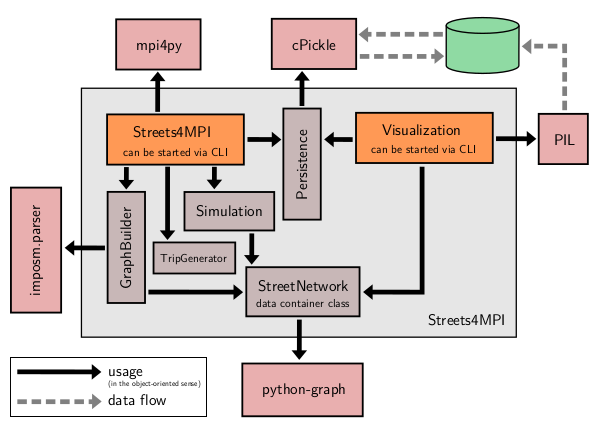
\includegraphics[width=.75\textwidth]{img/architecture_streets4mpi.png}
    \caption{Architecture overview: Streets4MPI~\cite[p. 9]{streets_report}}
    \label{fig:architecture_streets4mpi}
\end{figure}

The \textit{GraphBuilder} class parses \gls{osm} input data and builds a directed graph which is stored in the \textit{StreetNetwork}. The \textit{Simulation} than uses this data and repeatedly computes shortest paths for a set amount of \textit{trips} (randomly chosen node pairs from the graph). Over time it gradually modifies the graph based on results of previous iterations to emulate structural changes in the traffic network in the simulated area. The \texit{Persistence} class then optionally writes to results to a custom output format which is visualizable by an additional script~\cite{streets_report}.

\section{Differences and limitations}
\label{sec:Concept::Differences}

Although the evaluated applications are based on the original \textit{streets4MPI}, there are some key differences in the implementation. This section gives a brief overview over the most important aspects that have been changed. The first paragraph of each subsection describes the original application's functionality while the second highlights differences and limitations in the evaluated implementations.

In the remaining part of the thesis the different applications will be referenced quite frequently. For brevity the language implementations to compare will be called by the following scheme: ``streets4<language>''. The Go version for example is called ``streets4go''.

\subsection*{Input format}
\label{subsec:Concept::Differences::Input}

The original \textit{streets4MPI} uses the somewhat dated \gls{osm} \gls{xml} format\fnote{\url{http://wiki.openstreetmap.org/wiki/OSM_XML}} as input which is parsed by \textit{imposm.parser}\fnote{\url{http://imposm.org/docs/imposm.parser/latest/}}. It then builds a directed graph via the \textit{python-graph}\fnote{\url{https://code.google.com/p/python-graph/}} library to base the simulation on~\cite{streets_report}.

The derived versions require the input to be in ``.osm.pbf'' format. This newer version of the \gls{osm} format is based on Google's \gls{protobuf} and is superior to the \gls{xml} variant in both size and speed~\cite{osm_wiki_pbf}. It also simplifies multi language development because the code performing the actual parsing is auto generated from a language independent description file. There are \gls{protobuf} backends for C, Rust and Go which can perform that generation.

\subsection*{Simulation}
\label{subsec:Concept::Differences::Simulation}

The simulation in the base application is based on randomly picked node pairs from the source graph. For these trips the shortest path is calculated by Dijkstra's \gls{sssp} algorithm as seen in \cite{cormen}. Also a random factor called ``jam tolerance'' is introduced to avoid oscillation between two high traffic routes in alternating iterations~\cite{streets_report}. Then after some time has passed in the simulation, existing streets get expanded or shut down depending on their usage to simulate road construction.

The compared implementations of this thesis also perform trip based simulation but without the added randomness and street modification. Also the edge weights are not dynamically recalculated in each iterations. Instead the street's length is calculated once from the corrdinates of the corresponding nodes and used as edge weigth directly. The concrete algorithm is a variant of the \shinline{Dijkstra-NoDec} algorithm as seen in~\cite[p. 16]{dijkstra_utcs}. It was mainly chosen because of its reduced complexity in required data structures. The algorithm is implemented separately in all three languages so it could theoretically get benchmarked standalone to get clearer results. This was not attempted in scope of the thesis because of time constraints.

\subsection*{Concurrency}
\label{subsec:Concept::Differences::Concurrency}

\textit{streets4MPI} parallelizes its calculations on multiple processes that communicate via message passing. This is achieved with the aforementioned \textit{MPI4Py} library which delegates to a native \gls{mpi} implementation installed on the system. If no supported implementation is found it falls back to a pure Python solution. Results have show that the native one should be preferred in order to achieve maximum performance~\cite{streets_report}.

Although Rust as well as Go can integrate decently with existing native code, the reimplementations will be limited to shared memory parallelization on threads. This was mostly decided to evaluate and compare the language inherent concurrency constructs rather than the quality of their foreign funtion interfaces. To achieve a fair comparison \textit{streets4c} will use \textit{OpenMP}~\fnote{\url{http://www.openmp.org}} as it is the de facto standard for simple thread parallelization in C. Of course this solution might not match the performance of hand optimized implementations parallelized with the help of \textit{pthreads} but since the focus is on simple concurrency in the context of scientific applications \textit{OpenMP} was selected as the framework of choice.

\section{Implementation process}
\label{sec:Concept::Implementation}

The implementation process was performed iteratively. Certain milestones were defined and implemented in all three languages. The process only advanced to the next phase when the previous milestone was reached in all applications. This approach was chosen to allow for a fair comparison of the different phases of development. If the implementations would have been developed one after another to completion (or in any other arbitrary order), this might have introduced a certain bias to the evaluation because of possible knowledge about the problem aquired in a previous language translating to faster results in the next one.

\begin{figure}[htb]
    \centering
    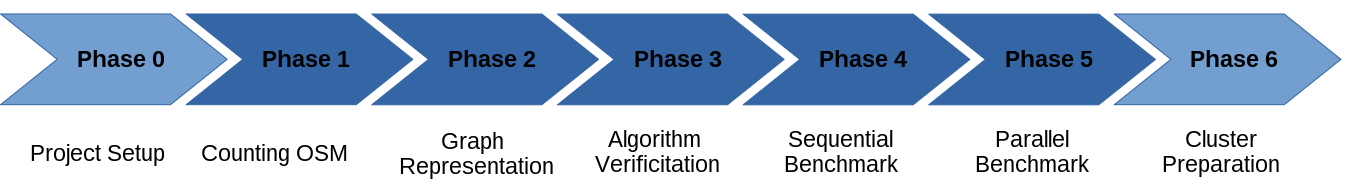
\includegraphics[width=\textwidth]{img/milestone_timeline.png}
    \caption{Milestone overview}
    \label{fig:milestone_timeline}
\end{figure}

\autoref{fig:milestone_timeline} shows the different milestones in order of completion. For each phase various characteristics were captured and compared to highlight the languages' features and performance in the various areas. While the main development and test runs were performed on a laptop the final application was run on a high performance machine provided by the research group Scientific Computing to compare scalability beyond common desktop level processors. In the following sections each milestone is briefly described.

\subsection*{Setting up the Project}
\label{subsec:Concept::Implementation::Setup}

The first phase of development was to create project skeletons and infrastructure for the future development. The milestone was to have a working environment in place where the sample application could be built and executed. While this is certainly not the most important or even interesting part it might show the differences in comfort between the various toolchains.

\subsection*{Counting Nodes, Ways and Relations}
\label{subsec:Concept::Implementation::Counting}

The first real milestone was to read a .osm.pbf file and count all nodes, ways and relations in it. This was done to get familiar with the required libraries and the file format in general. The time recorded began from the initial project created in phase 0 and finished after the milestone was reached. As this is the most input and output intensive phase it should reveal some key differences between the candidates both in speed as well as memory consumption.

\subsection*{Building a basic Graph Representation}
\label{subsec:Concept::Implementation::Graph_Representation}

The next goal was to conceptionally build the graph and related structures the simulation would later operate on. This involved thinking about the relation between edges and nodes as well as the choice of various containers to store the objects efficiently while also keeping access simple. In addition the shortest path algorithm had to be implemented. This meant a priority queue had to be available as the algorithm relies on that data structure to store nodes which have yet to be processed. This milestone therefore tested the language's standard libraries and expressiveness in terms of typed containers.

\subsection*{Verifying Structure and Algorithm}
\label{subsec:Concept::Implementation::Verification}

After the base structure to represent graphs and calculate shortest paths was in place it was time to validate the implementations. Unfortunately the OSM data used in the first phase contained too much nodes and ways to be able to efficiently verify any computed results. Therefore a small example graph was manually populated and fed to the algorithm.

\subsection*{Benchmarking Graph Performance}
\label{subsec:Concept::Implementation::SequentialBenchmark}

The fourth milestone was preliminary benchmark of the implementations. The basic idea was to parse the \gls{osm} data used in phase one and build the representing graph. After that the shortest path algorithm is executed once for each node. The total execution time as well as the time taken for each step (building the graph and calculating shortest paths) should be measured and compared as well as the usual memory statistics from previous phases.

\subsection*{Benchmarking Parallel Execution}
\label{subsec:Concept::Implementation::ParallelBenchmark}

The fifth phase consisted of modifying the existing benchmark to operate in parallel via threading and benchmarking the results for various configurations. While all the development and previous benchmarks were performed on a personal laptop the final benchmarks were taken on a computation node of the research group to gather relevant results in high concurrency situations.

\subsection*{Cluster Preperation}
\label{subsec:Concept::Implementation::ClusterPreparation}

The final milestone was to prepare the implementations for the execution on the cluster provided by the research group. As this was a remote environment with some key differences to the development laptop the implementations had to be prepared and slightly changed.

\section{Overview of evaluated Criteria}
\label{sec:Concept::Criteria}

For the evaluation of the three languages multiple criteria have been selected. While some of them are directly quantifiable such as development time others are rated subjectively based on experiences from the implementation process. This is mostly true for the productivity metrics. It is important to note that not all statistics apply to all milestones. The following list introduces the reviewed criteria and briefly describes them.
\\

\begin{itemize}
    \item Performance
    \begin{itemize}
        \item Execution Time\\
        \textit{The time to complete the task of the milestone}
        \item Memory Footprint\\
        \textit{Total memory consumption as well as allocation and free counts}
    \end{itemize}
    \item Productivity
    \begin{itemize}
        \item \acrshort{sloc} Count\\
        \textit{Source lines of code to roughly estimate the code's complexity and maintainability. Tracked in all milestones}
        \item Development Time\\
        \textit{Time required to implementation the desired functionality. Tracked in all milestones}
        \item Tooling Support\\
        \textit{Tooling support for common tasks throughout the development process. This includes the compiler, dependency management, project setup automation and many more}
        \item Library Ecosystem\\
        \textit{Available libraries for the given language considering common data structures, algorithms or mathematical functions. Includes the quality of the language's standard library}
        \item Parallelization Effort\\
        \textit{Amount of work required to parallelize an existing sequential application}
    \end{itemize}
\end{itemize}

As these statistics were tracked during the implementation itself the \hyperref[ch:Implementation]{next chapter} directly lists and evaluates intermediate results for each milestone. In contrast \autoref{ch:Evaluation} evaluates the final performance outcomes from the cluster benchmarks as well as the gathered productivity metrics.

\section{Related Work}
\label{sec:Concept::Related}

The search for new programming languages which are fit for \gls{hpc} is not a recently developing trend. There have been multiple studies and evaluations but so far none of the proposed languages have gained enough traction to receive widespread adoption. Also most reports focused on the execution performance without really considering additional software metrics or developer productivity. \cite{related_multicore} adds lines of code and development time to the equation but both of these metrics only allow for superficial conclusions about code quality and productivity.

From the candidates presented here Go in particular has been compared to traditional \gls{hpc} languages with mixed results. Although its regular execution speed is somewhat lacking \cite{related_sor_study} showed the highest speedup from parallelization amongst the evaluated languages which is very promising considering high concurrency scenarios like cluster computing. Rust on the other hand has not been seriously evaluated in the \gls{hpc} context probably due to it still being developed.
